\documentclass[10pt]{beamer}

\usetheme[progressbar=frametitle]{metropolis}

\usepackage{appendixnumberbeamer}

\usepackage{booktabs}
\usepackage{blkarray}
%\usepackage{ccicons}
\usepackage{graphicx}
\usepackage{color}

\definecolor{UniBlue}{RGB}{7,82,154}
\definecolor{UniYellow}{RGB}{234,185,12}

%\setbeamercolor{title}{fg=UniBlue, bg = UniYellow}
%\setbeamercolor{frametitle}{fg=UniBlue, bg= UniYellow}
%\setbeamercolor{structure}{fg=UniBlue, bg= UniYellow}
%\setbeamercolor{progress bar}{fg=UniBlue, bg= UniYellow}
\usepackage{xspace}

\title{Multiscale testing for equality of nonparametric trend curves}
\date{November 26, 2021\\ Workshop on panel data \\ Tinbergen Institute \& University of Amsterdam}
\author{Marina Khismatullina \and Michael Vogt}
\setbeamertemplate{frame footer}{Multiscale inference for nonparametric time trends}
\metroset{block=fill}
% \titlegraphic{\hfill\includegraphics[height=1.5cm]{logo.pdf}}

\newcommand{\Prob}{\mathrm{P}}
\newcommand{\E}{\mathbb{E}}
\newcommand{\Eps}{\mathcal{E}}
\newcommand{\eps}{\varepsilon}
\newcommand{\reals}{\mathbb{R}}
\newcommand{\X}{\boldsymbol{X}}
\newcommand{\bfbeta}{\boldsymbol{\beta}}
\newcommand{\Var}{\mathrm{Var}}
\newcommand{\Cov}{\mathrm{Cov}}
\newcommand{\Corr}{\mathrm{Corr}}
\newcommand{\sgn}{\text{sgn}}
\newtheorem{prop}{Proposition}
\newcommand{\ind}{\boldsymbol{1}\Big( \frac{t}{T} \in \mathcal{I}_k \Big)} % indicator function
\newcommand{\indsmall}{\boldsymbol{1}\big( \frac{t}{T} \in \mathcal{I}_k \big)} % indicator function

\begin{document}

\maketitle

\begin{frame}{Table of contents}
  \setbeamertemplate{section in toc}[sections numbered]
  \tableofcontents[hideallsubsections]
\end{frame}

\section{Introduction}


\begin{frame}{Motivation}

{\onslide<1-> \begin{block}{Aim of the paper}
	To develop new inference methods that allow to \textit{identify} and \textit{locate} differences between nonparametric trend curves with dependent errors.
\end{block}}
	{\onslide<2>\begin{figure}
    		\centering
    		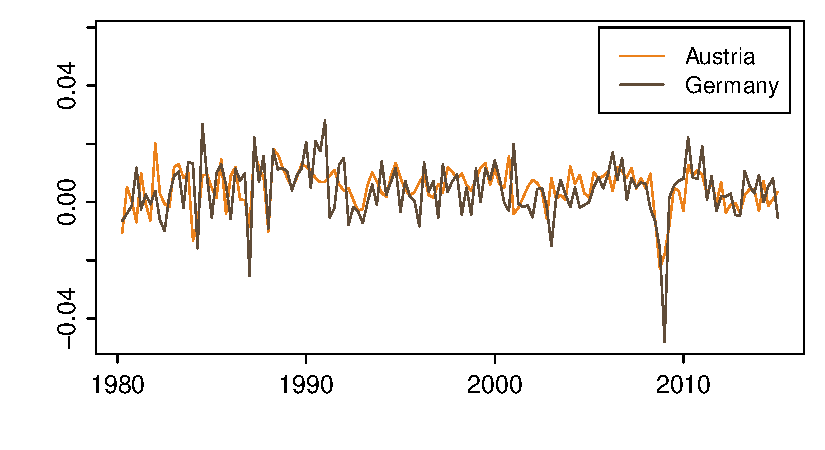
\includegraphics[height=0.45\textheight]{plots/gdp_AUT_DEU.pdf}
  	\end{figure}}
	{\onslide<3>
	\vspace{-46,81mm}
	\begin{figure}
    		\centering
    		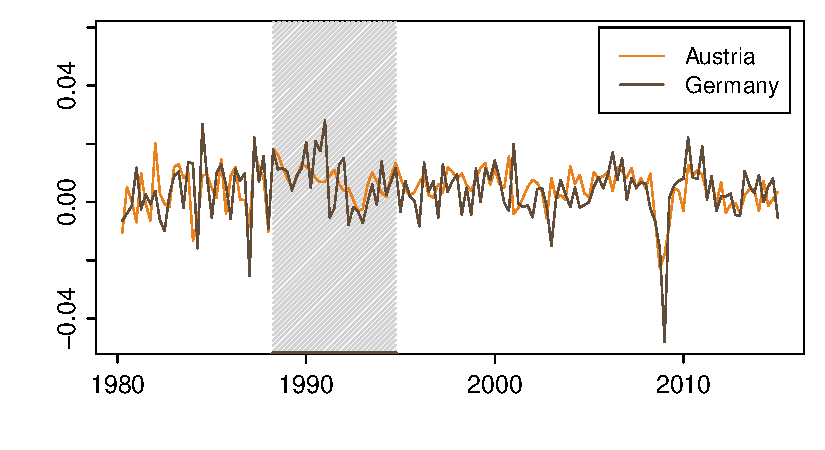
\includegraphics[height=0.45\textheight]{plots/gdp_AUT_DEU_1.pdf}
  	\end{figure}}	
	{\onslide<4->
	\vspace{-46,81mm}
	\begin{figure}
    		\centering
    		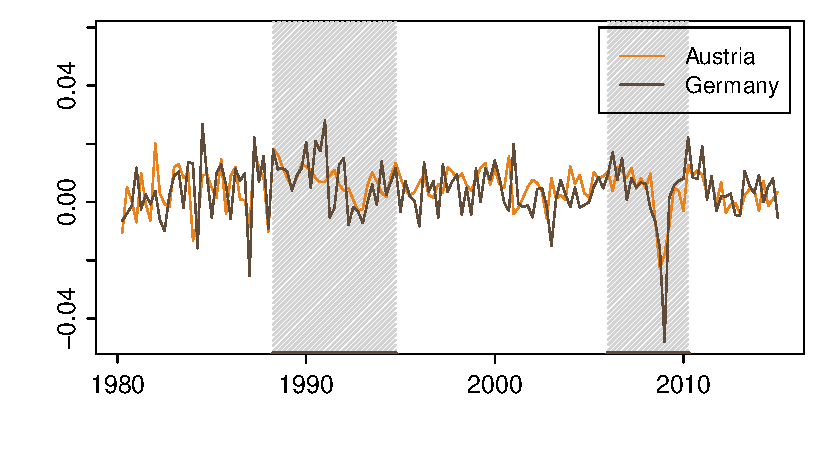
\includegraphics[height=0.45\textheight]{plots/gdp_AUT_DEU_2.pdf}
  	\end{figure}}	
\vspace{-3mm}
{\onslide<5->\textbf{Research question:}
	Out of many given intervals, how to find those where the trends are significantly different?}


%\textbf{Aim:} to compare the underlying trends on different intervals simultaneously.}
\end{frame}

\begin{frame}{Motivation}
\vspace{-4mm}
\textbf{Why is it relevant?}

Finding systematic differences between trends = basis for further research.\pause

%$\quad \quad \Rightarrow$ understanding which government policies are more effective.\pause

\vspace{3mm}

\textbf{Why is it difficult?}	

Testing many hypotheses at the same time = multiple testing problem

$\quad \quad \Rightarrow$ large probability of one true null hypothesis being rejected.\pause

\vspace{3mm}

\textbf{Is it limited to a particular application?}

No! Our method = general method for comparing nonparametric trends

$\quad \quad \Rightarrow$ new statistical test for equality of nonparametric trend curves.
 
\end{frame}

\begin{frame}{Literature}
	Comparison of deterministic trends:
	\begin{itemize}
		\item {\color<2>{mLightBrown}Park et al. (2009)}, Degras et al. (2012), Zhang et al. (2012), Hidalgo and Lee (2014), Chen and Wu (2019).
	\end{itemize}\pause\pause
	Multiscale tests:
	\begin{itemize}
		\item Chaudhuri and Marron (1999, 2000), Hall and Heckman (2000), D{\"u}mbgen and Spokoiny (2001), {\color<4>{mLightBrown}Park et al. (2009)}, Khismatullina and Vogt (2020).
	\end{itemize}\pause
%	\pause
%	Comparison of volatility trends:
%	\begin{itemize}
%		\item Nyblom and Harvey (2000), ...
%	\end{itemize}
\end{frame}


\section{Model}

\begin{frame}{Model}
We observe a panel of $n$ time series $\mathcal{Z}_i = \{(Y_{it}, \X_{it}): 1 \le t \le T \}$ of length $T$, where $Y_{it} \in \reals$ and $\X_{it}\in \reals^{d}$. \pause We assume that $n$ is fixed. \pause

We consider the following model:
\begin{equation*}
Y_{it} = m_i \Big( \frac{t}{T} \Big) + \bfbeta_i^T\X_{it}+ \alpha_i + \varepsilon_{it},
\end{equation*}\pause
\vspace{-3mm}
where
\begin{itemize}
\item $m_i$ are unknown trend functions on $[0,1]$;\pause
\item $\bfbeta_i$ is $d\times 1$ vector of unknown parameters;\pause
\item $\alpha_i$ are so-called fixed effect error terms;\pause
\item $\Eps_i = \{\eps_{it}: 1\leq t \leq T\}$ is a zero-mean stationary and causal error process.
\end{itemize}
\end{frame}

\begin{frame}{Model, part 2}
\begin{equation*}
Y_{it} = m_i \Big( \frac{t}{T} \Big) + \bfbeta_i^T\X_{it}+ \alpha_i + \varepsilon_{it},
\end{equation*}\pause
If we knew $\alpha_i$ and $\bfbeta_i$, then the model becomes much simpler:
\begin{align*}
Y_{it} - \alpha_i - \bfbeta_i^\top \X_{it} & =: Y_{it}^\circ\\
					& = m_i \Big( \frac{t}{T} \Big) + \varepsilon_{it}. 
\end{align*}\pause
In reality the variables $Y_{it}^\circ$ are \textbf{not} observed. \pause

But given $\widehat{\alpha}_i$ and $\widehat{\bfbeta}_i$, we can consider
\begin{align*}
	\widehat{Y}_{it} := Y_{it} -\widehat{\alpha}_i - \widehat{\bfbeta}_i^\top \X_{it} =(\bfbeta_i - \widehat{\bfbeta}_i)^\top \X_{it} + m_i \Big( \frac{t}{T} \Big) + \big( \alpha_i - \widehat{\alpha}_i \big) + \varepsilon_{it}. 
\end{align*}
\end{frame}


\begin{frame}{Model, part 3}
1. We estimate $\bfbeta_i$:
\begin{align*}
\widehat{\bfbeta}_i = \Big( \sum_{t=2}^T \Delta \X_{it} \Delta \X_{it}^\top \Big)^{-1} \sum_{t=2}^T \Delta \X_{it} \Delta Y_{it}
\end{align*}\pause
\vspace{-3mm}
\begin{block}{Theorem}
Under certain regularity assumptions, $\widehat{\bfbeta}_i$ is a consistent estimator of $\bfbeta_i$ with the property $\bfbeta_i - \widehat{\bfbeta}_i = O_P(T^{-1/2})$.
\end{block}\pause
2. We estimate the fixed effects $\alpha_i$:
\begin{align*}
\widehat{\alpha}_i &= \frac{1}{T}\sum_{t=1}^T \big(Y_{it} - \widehat{\bfbeta}_i^\top \X_{it}\big)
\end{align*}\pause
We then work with the augmented time series \color{mLightBrown}{$\widehat{Y}_{it} = Y_{it} - \widehat{\alpha}_i - \widehat{\bfbeta}_i^\top \X_{it}$}.
\end{frame}

\begin{frame}{Original time series: Austria and Germany}
\begin{figure}
    		\centering
    		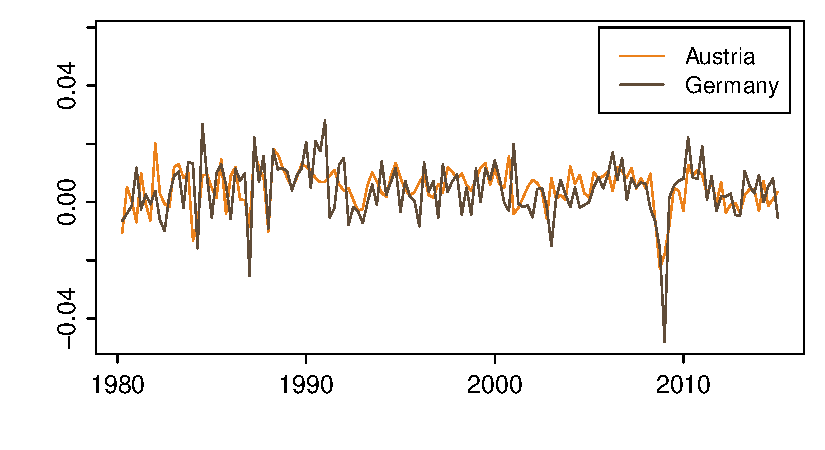
\includegraphics[height=0.65\textheight]{plots/gdp_AUT_DEU.pdf}
  	\end{figure}
\end{frame}

\begin{frame}{Augmented time series: Austria and Germany}
	\begin{figure}
    		\centering
    		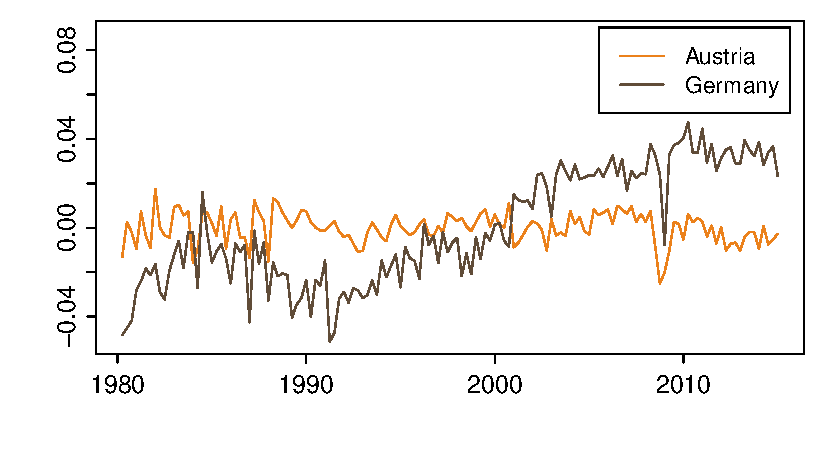
\includegraphics[height=0.65\textheight]{plots/gdp_AUT_DEU_adj.pdf}
  	\end{figure}	
\end{frame}


\begin{frame}{Original time series: Canada and USA}
\begin{figure}
    		\centering
    		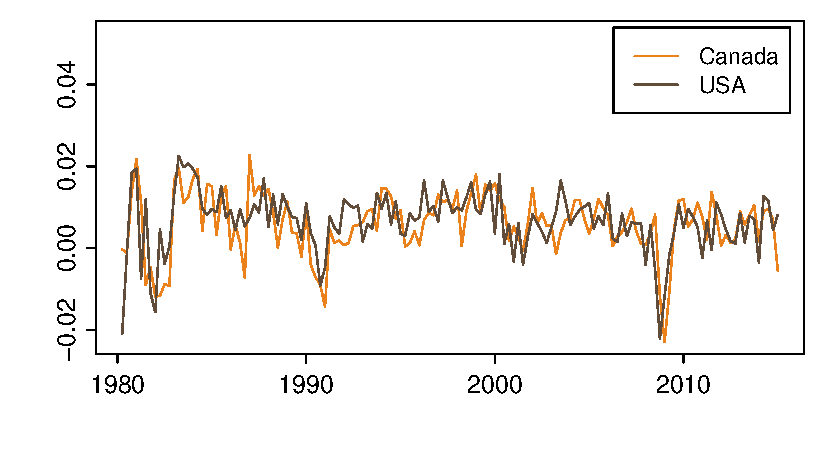
\includegraphics[height=0.65\textheight]{plots/gdp_CAN_USA.pdf}
  	\end{figure}
\end{frame}

\begin{frame}{Augmented time series: Canada and USA}
	\begin{figure}
    		\centering
    		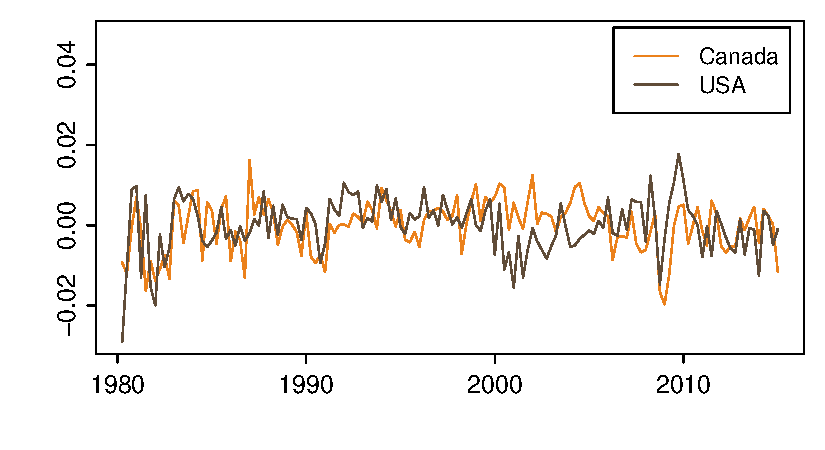
\includegraphics[height=0.65\textheight]{plots/gdp_CAN_USA_adj.pdf}
  	\end{figure}	
\end{frame}


\section{Testing procedure}

\begin{frame}{Testing problem}

\begin{align*}
H_0: m_1 = m_2 = \ldots = m_n
\end{align*}\pause

\vspace{-4mm}
\textbf{Question}: if we reject the global null, how to locate the differences between the trends? \pause

Consider a grid $\mathcal{G}_T = \{(u, h): [u-h, u+h] \subseteq [0, 1]\}$ of location-bandwidth parameters. \pause For each pair $(i, j)$ and for each interval $[u-h, u+h]$ we consider the null hypothesis 
\[ H_0^{[i,j]}(u,h): m_i(w) = m_j(w) \text{ for all } w \in [u-h,u+h]. \]\pause
Then the global null $H_0: m_1 = m_2 = \ldots = m_n$ can be reformulated as
\begin{align*}
H_0:  &\text{The hypotheses } H_0^{[i,j]}(u,h) \text{ hold true for all intervals } \\ &[u- h , u+h], (u, h) \in \mathcal{G}_T, \text{ and for all } 1 \le i < j \le n. 
\end{align*} 
\end{frame}


\begin{frame}{Test statistic}
For a given location $u \in [0,1]$ and bandwidth $h$ and a given pair $(i, j)$ we construct the kernel averages
\begin{equation*}
\widehat{\psi}_{ij, T}(u,h) = \sum\limits_{t=1}^T w_{t,T}(u,h) \big(\widehat{Y}_{it} - \widehat{Y}_{jt}), 
\end{equation*}\pause
\vspace{-3mm}
where 
\begin{align*}
w_{t,T}(u,h) &= \frac{\Lambda_{t,T}(u,h)}{ \{\sum\nolimits_{t=1}^T \Lambda_{t,T}^2(u,h)\}^{1/2} } ,\\
\Lambda_{t,T}(u,h) &= K\Big(\frac{t/T-u}{h}\Big) \Big[ S_{T,2}(u,h)  - S_{T,1}(u,h)\Big(\frac{t/T-u}{h}\Big) \Big], \\
S_{T,\ell}(u,h) &= \frac{1}{Th} \sum\nolimits_{t=1}^T K\Big(\frac{t/T-u}{h}\Big) \Big(\frac{t/T-u}{h}\Big)^\ell
\end{align*}
for $\ell = 1,2$ and $K$ is a kernel function.
\end{frame}

\begin{frame}[label = frame_teststatistic]{Test statistic, part 2}
The kernel averages $\widehat{\psi}_{ij, T}(u,h)$ measure the distance between two trend curves $m_i$ and $m_j$ on $[u - h, u + h]$. \pause

Instead with working directly with $\widehat{\psi}_{ij, T}(u,h)$, we replace them by
\begin{equation*}
\widehat{\psi}^0_{ij, T}(u,h) = \bigg\{ \bigg|\frac{\widehat{\psi}_{ij, T}(u,h)}{\big(\widehat{\sigma}_i^2 + \widehat{\sigma}_j^2\big)^{1/2}}\bigg| - \lambda(h) \bigg\}, 
\end{equation*}\pause
\vspace{-3mm}
%Test statistic is defined as follows
%\begin{equation*}
%\widehat{\Psi}_T = \max_{(u,h) \in \mathcal{G}_T} \Big\{ \Big|\frac{\widehat{\psi}_T(u,h)}{\widehat{\sigma}}\Big| - \lambda(h) \Big\}, 
%\end{equation*} \pause
where 
\begin{itemize}
\item $\widehat{\sigma}_i^2$ is an appropriate estimator of the long-run variance $\sigma^2_i$;\pause
\item $\lambda(h) = \sqrt{2 \log \{ 1/(2h) \}}$ is an additive correction term (D{\"u}mbgen and Spokoiny (2001)). %\hyperlink{frame_lambda}{\beamerbutton{Explanation}}
\end{itemize}
\end{frame}

\begin{frame}{Test statistic, part 3}

To test the global null, we aggregate the individual test statistics \linebreak for all $(i, j)$ and all location-bandwidth pairs $(u, h) \in \mathcal{G}_T$:
\begin{equation*}
\widehat{\Psi}_{n, T} = \max_{1 \leq i < j \leq n} \max_{(u,h) \in \mathcal{G}_T} \widehat{\psi}^0_{ij, T}(u,h). 
\end{equation*}\pause
\vspace{-3mm}
\begin{block}{Main theoretical result}
Under certain conditions and under the null, $\widehat{\psi}^0_{ij, T}(u,h)$ and $\widehat{\Psi}_{n, T}$ can be approximated by the corresponding Gaussian versions of the test statistics.
\end{block}
\end{frame}

\begin{frame}{Test procedure}
Gaussian version of the individual test statistics:
\begin{align*}
{\phi}^0_{ij, T}(u,h) = \max_{(u,h) \in \mathcal{G}_T} \bigg\{ \bigg|\frac{\phi_{ij, T}(u,h)}{\big(\sigma^2_i + \sigma^2_j\big)^{1/2}}\bigg| - \lambda(h) \bigg\},
\end{align*} \pause
\vspace{-3mm}
where
\begin{itemize}
\item $\phi_{ij, T}(u,h) = \sum\nolimits_{t=1}^T w_{t,T}(u,h) \, {\color<3>{mLightBrown}\big\{\sigma_i(Z_{it} - \bar{Z}_i) - \sigma_j(Z_{jt} - \bar{Z}_j)\big\}}$;\pause\pause
\item $Z_{it}$ are independent (across $i$ and $t$) standard normal random variables;\pause
\item $\bar{Z}_i$ is the empirical average of $Z_{i1}, \ldots, Z_{iT}$.
\end{itemize}\pause


Aggregated Gaussian test statistics:
\begin{equation*}
\Phi_{n, T} = \max_{1 \leq i < j \leq n} \max_{(u,h) \in \mathcal{G}_T} \phi^0_{ij, T}(u,h). 
\end{equation*}

\end{frame}

\begin{frame}[label = frame_test]{Test procedure, part 2}

\begin{enumerate}
	\item Consider the Gaussian test statistic 
	\vspace{-2mm} \[ \Phi_{n, T} = \max_{1 \leq i < j \leq n} \max_{(u,h) \in \mathcal{G}_T} \phi^0_{ij, T}(u,h), \] where $\phi^0_{ij, T}$ are weighted averages of the differences of standard normal random variables.\pause
	\item Compute a $(1-\alpha)$-quantile $q_{n, T} (\alpha)$ of $\Phi_{n,T}$ by Monte Carlo simulations.\pause
	\item Perform the test for the global hypothesis $H_0$: reject $H_0$ if $\widehat{\Psi}_{n, T} > q_{n, T}(\alpha)$.\pause
	\item For each $i, j$, and each $(u, h) \in \mathcal{G}_T$, carry out the test for the local null hypothesis $H^{[i,j]}_0(u, h)$: reject $H^{[i,j]}_0(u, h)$ if $\widehat{\psi}^0_{ij, T}(u, h) > q_{n, T}(\alpha)$.
	\end{enumerate}
\end{frame}


\section{Theoretical properties}




\begin{frame}[label = frame_assumptions]{Assumptions}
\begin{itemize}

\item[$\mathcal{C}1$] \label{C-err1} For all $i$ it holds that $\E[\varepsilon_{it}] =0$ and $\| \varepsilon_{it} \|_q < \infty$ for some $q > 4$.\pause
\item[$\mathcal{C}2$] For each $i$ the variables $\varepsilon_{it}$ are weakly dependent. \hyperlink{tech_assumptions}{\beamerbutton{Details}}\pause

\item[$\mathcal{C}3$] \label{C-reg} For each $i$ we have that $\X_{it}$ is stationary and causal with all the necessary moments and no asymptotic multicollinearity.\pause

\item[$\mathcal{C}4$] For each $i$ the variables $\X_{it}$ are weakly dependent. \hyperlink{tech_assumptions_2}{\beamerbutton{Details}}\pause
\item[$\mathcal{C}5$]  $\X_{it}$ (elementwise) and $\varepsilon_{is}$ are uncorrelated for each $t, s$.\pause

\item[$\mathcal{C}6$] All of the variables in the model are short-range dependent.\hyperlink{tech_assumptions_3}{\beamerbutton{Details}}

\end{itemize}
\end{frame}

\begin{frame}{Assumptions, part 2}
\begin{itemize}
\item[$\mathcal{C}7$]\label{C-ker} Standard assumptions on the kernel function $K$. \pause
\item[$\mathcal{C}8$] \label{C-grid} $|\mathcal{G}_T| = O(T^\theta)$ for some arbitrarily large but fixed constant $\theta > 0$.\pause
\begin{align*}
\mathcal{G}_T = \big\{ & (u,h): u = t/T \text{ for some } 1 \le t \le T \text{ and } h \in [h_{\min},h_{\max}] \\ & \text{ with } h = t/T \text{ for some } 1 \le t \le T  \big\},
\end{align*}\pause
\vspace{-5mm}
\item[$\mathcal{C}9$] \label{C-h} $h_{\min} \gg T^{-(1-\frac{2}{q})} \log T$ and $h_{\max} <1/2$.\pause
\item[$\mathcal{C}10$] Assume that $\sigma_i^2 = \sigma_j^2$ for all $i, j$ and $\widehat{\sigma}_i^2 = \sigma_i^2 + o_p(\rho_T)$ with $\rho_T = o(\sqrt{h_{\min}}/\log T)$.
\end{itemize}
\end{frame}

\begin{frame}{Theoretical properties}
\begin{prop} Under $\mathcal{C}1 - \mathcal{C}10$ and under the null, it holds that 
\vspace{-2mm}
\begin{align*}
\Prob\Big(\widehat{\Psi}_{n, T} \leq q_{n, T}(\alpha)\Big) = 1 - \alpha + o(1)
\end{align*}
\vspace{-5mm}
\end{prop} \pause
\begin{corollary} $$\text{FWER}(\alpha)\leq \alpha$$
\end{corollary} \pause
\begin{prop}\label{prop2}
Consider a sequence of functions $m_{i} = m_{i,T}$, $m_{j} = m_{j, T}$ such that 
\begin{equation*}
\exists \, (u, h)\in \mathcal{G}_{T}:  m_{i}(w) - m_{j}(w) \ge c_T \sqrt{\log T / (T h)} \,\, \forall w \in [u-h, u+h],
\end{equation*} and $c_T \rightarrow \infty$. Then under $\mathcal{C}1 - \mathcal{C}10$, it holds that
\vspace{-2mm}
\begin{equation*}
\Prob\Big( \widehat{\Psi}_{n, T} \leq q_{n, T}(\alpha)\Big) = o(1)
\end{equation*}
\vspace{-5mm}
\end{prop}
\end{frame}





%\begin{frame}[label = frame_critval]{Critical values}
%How to construct critical values $c_{ijk}(\alpha)$?\pause
%\begin{itemize} 
%\item Traditional approach: $c_{ijk}(\alpha) = c(\alpha)$ for all $(i,j,k)$. \pause
%\item More modern approach: $c_{ijk}(\alpha)$ depend on the length $h_k$ of the time interval (D{\"u}mbgen and Spokoiny (2001))\pause:
%\[c_{ijk}(\alpha) = c(\alpha,h_k) := b_k + q(\alpha)/a_k,\] where $a_k$ and $b_k$ are scale-dependent constants and $q(\alpha)$ is chosen such that we control FWER.
%\hyperlink{frame_scaleconstants}{\beamerbutton{Details}}
%\end{itemize}
%\end{frame}
%
%
%\begin{frame}{Critical values, part 2}
%We want to control FWER. \pause Let $\mathcal{M}_0: = \big\{(i, j, k) | H_0^{(ijk)} \text{ is true} \big\}$, then
%\begin{align*}
%\text{FWER}(\alpha) &= \Prob \Big( \exists (i,j,k) \in \mathcal{M}_0:  |\widehat{\psi}_{ijk} | > c_{ijk}(\alpha) \Big) \\
%\onslide<3->{&= 1 - \Prob \Big( \forall (i,j,k) \in \mathcal{M}_0: |\widehat{\psi}_{ijk} | \le c_{ijk}(\alpha) \Big)}\\
%\onslide<4->{& =  1 - \Prob \Big( \forall (i,j,k) \in \mathcal{M}_0: a_k \big(|\hat{\psi}_{ijk}| - b_k\big) \le q(\alpha) \Big)}\\
%\onslide<5->{& = 1 - \Prob\Big( \max_{(i,j,k) \in \mathcal{M}_0} a_k \big( |\hat{\psi}_{ijk}| - b_k \big) \le q(\alpha) \Big)}\\
%\onslide<6->{ & \leq 1 - \Prob\Big( \max_{(i,j,k)} a_k \big( |{\color<7>{mLightBrown}\hat{\psi}_{ijk}^0}| - b_k \big) \le q(\alpha) \Big)}
%\end{align*}
%\onslide<8->{Hence, we choose $q(\alpha)$ as the $(1-\alpha)$-quantile of the statistic 
%\[ \hat{\Psi}_T = \max_{(i,j,k)} a_k \big( |\hat{\psi}_{ijk}^0| - b_k \big), \]
%where $\hat{\psi}_{ijk}^0$ is equal to $\hat{\psi}_{ijk}$ under the null.}
%\end{frame}
%
%\begin{frame}{Critical values, part 3}
%
%But we do not know the distribution of $\hat{\Psi}_T$ in practice!\pause
%
%$\Rightarrow$ the quantiles $q(\alpha)$ are also not known. How to approximate them?\pause
%
%Under our assumptions, 
%\[ \hat{\psi}_{ijk}^0 \approx \frac{1}{\sqrt{2 T h_k}} \sum\limits_{t=1}^T \ind  (\eta_{it} - \eta_{jt} ), \] \pause
%which can be approximated by a Gaussian version of the test statistic:
%\begin{align*}
%\phi_{ijk} = \frac{1}{\sqrt{2 T h_k}} \sum\limits_{t=1}^T \ind (Z_{it} - Z_{jt}), 
%\end{align*}
%where $Z_{it}$ are independent standard normal random variables.
%
%
%\end{frame}




\section{Illustration}

\begin{frame}{Graphical representation}
How to represent the results of the test? \pause

We can plot all of the intervals where we reject the local null. \pause

But what if there are too many?\pause

An interval $[u-h, u+h]$ is called \textbf{minimal} if the corresponding local null $H_0^{[i,j]}(u,h)$ is rejected and there is no other interval $[u^\prime-h^\prime, u^\prime+h^\prime]$ such that we reject $H_0^{[i,j]}(u^\prime,h^\prime)$ and $[u^\prime-h^\prime, u^\prime+h^\prime] \subset [u-h, u+h]$.

\end{frame}

%\begin{frame}{Graphical representation}
%How to represent the results of the test? \pause
%
%For each pair of time series $(i, j)$, denote by $\mathcal{S}^{[i, j]}(\alpha)$ the set of intervals $[u-h, u+h]$ that consists of the intervals where we reject $H_0^{[i,j]}(u,h)$ at a significance level $\alpha$.\pause
%\begin{align*}\Prob\Big(& \forall \, i,j \in \{1, \ldots, n\}, (u, h) \in \mathcal{G}_T \text{ such that }\\
%&H_0^{[i, j]}(u, h) \text{ is true}: |\hat{\psi}^0_{ij,T}(u, h)| \le q_{n,T}(\alpha) \Big) \ge 1 - \alpha + o(1)
%\end{align*}
%\pause
%\vspace{-3mm}
%\begin{block}{Minimal intervals}
%An interval $[u-h, u+h] \in \mathcal{S}^{[i, j]}$ is called \textbf{minimal} if there is no other interval $[u^\prime-h^\prime, u^\prime+h^\prime] \in  \mathcal{S}^{[i, j]}$ with $[u^\prime-h^\prime, u^\prime+h^\prime] \subset [u-h, u+h]$.
%\end{block}
%\end{frame}

%\begin{frame}{Application setting}
%\begin{itemize}
%\item Five countries: Germany, Italy, Spain, France and the UK.
%\item $T = 150$ days. 
%\item The data is aligned by weekdays: first Monday after reaching $100$ cases as $t=1$.
%\item Lengths of time intervals $7, 14, 21, 28$ days. The intervals start at days $1, 8, 15, \ldots$ and $4, 11, 19, \ldots$
%\item $\alpha = 0.05$.
%\item $5000$ Monte Carlo simulation runs to produce critical values.
%\end{itemize}
%\end{frame}
%
\begin{frame}{Application results}
	\begin{figure}
		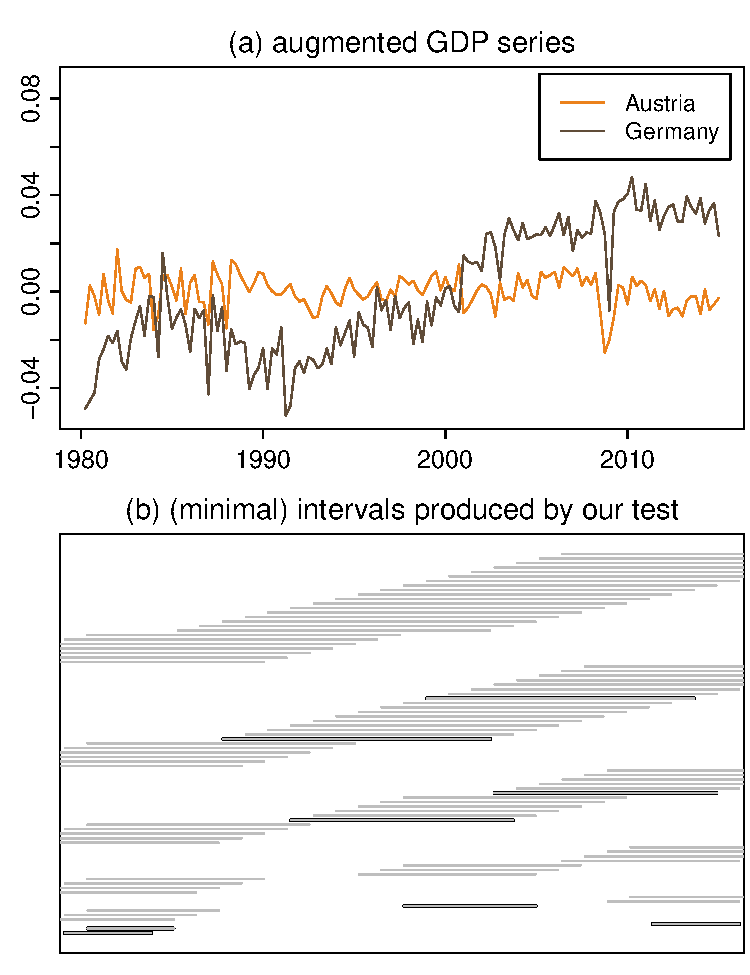
\includegraphics[width=0.49\textwidth]{plots/gdp_AUT_vs_DEU_talk}
   		%\caption{Observed new cases per day in Germany and Italy}    			\label{fig:DEUvsITA}
		\hfill
		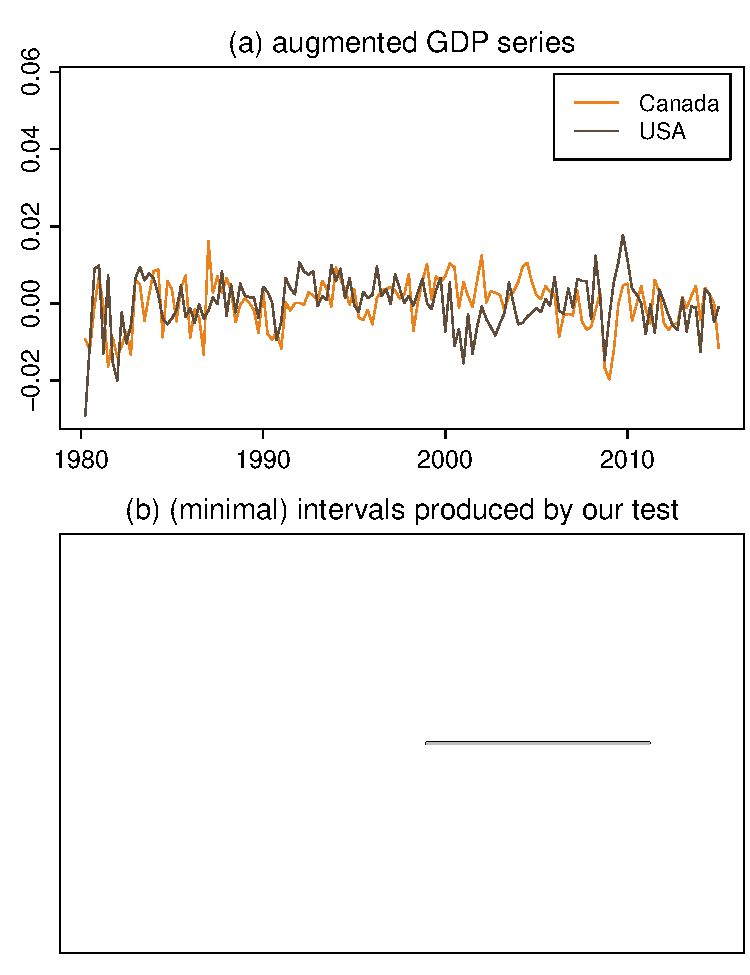
\includegraphics[width=0.49\textwidth]{plots/gdp_CAN_vs_USA_talk}
	\end{figure}
\end{frame}

%\begin{frame}{Application results, part 2}
%	\begin{figure}
%		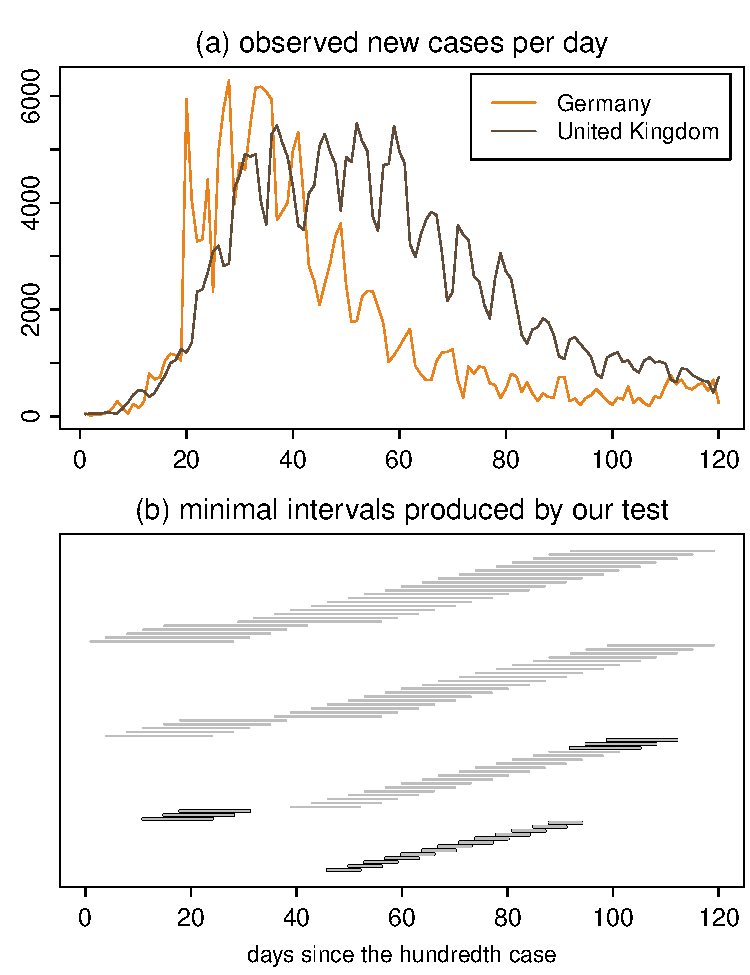
\includegraphics[width=0.49\textwidth]{plots/DEU_vs_GBR_presentation}
%   		%\caption{Observed new cases per day in Germany and Italy}    			\label{fig:DEUvsITA}
%		\hfill
%		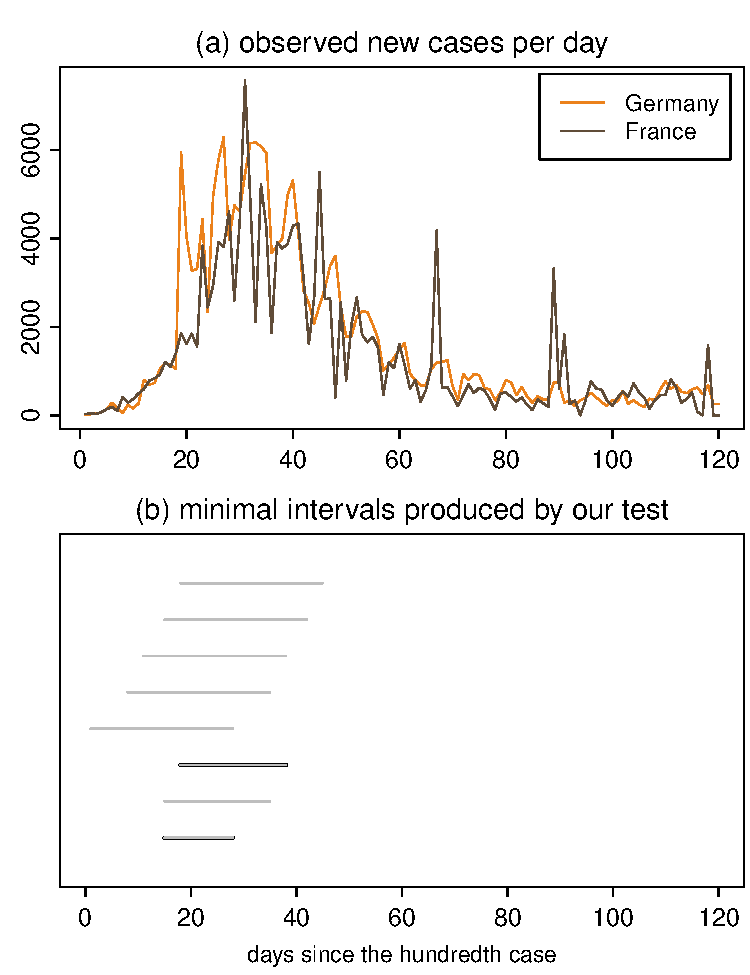
\includegraphics[width=0.49\textwidth]{plots/DEU_vs_FRA_presentation}
%	\end{figure}
%\end{frame}


\begin{frame}{Discussion}
We can claim, with confidence of at least $95\%$, that the null hypothesis is violated for all intervals (and all pairs of time series) for which our test rejects the null. \pause

However, we can not say anything about the causes of such differences. This question requires further (probably not purely statistical) analysis.\pause

Further possible extensions:
\vspace{-1mm}
\begin{itemize}
	\item introduce scaling factor in the trend function;\pause
	\item include the dependence between covariates and error terms;\pause
	\item cluster the time series based on the trends they exhibit.
\end{itemize}
\end{frame}

\begin{frame}[standout]
  Thank you!
\end{frame}


\appendix

\begin{frame}{Strategy of the proof}
\begin{itemize}
\item Introduce $\widehat{\Phi}_{n, T}$ that is close in distribution to $\widehat{\Psi}_{n, T}$ under the null.\pause
\item Using strong approximation theory for dependent processes as derived in Berkes et al. (2014), replace $\widehat{\Phi}_{n, T}$ by $\widetilde{\Phi}_{n, T}$ with the same distribution and the property that 
\begin{equation*}\label{eq-theo-stat-strategy-step1}
\big| \widetilde{\Phi}_{n, T} - \Phi_{n, T} \big| = o_p(\delta_T),
\end{equation*}
where $\delta_T$ goes to $0$ as $T\to\infty$ sufficiently fast.\pause
\item Using the anti-concentration results for Gaussian random vectors (Chernozhukov et al. 2015), prove that $\Phi_{n, T}$ does not concentrate too strongly in small regions of the form $[x-\delta_T,x+\delta_T]$, i.e.
\begin{equation*}\label{eq-theo-stat-strategy-step2}
\sup_{x \in \mathbb{R}} \Prob \big( |\Phi_{n, T} - x| \le \delta_T \big) = o(1).
\end{equation*}\pause
\vspace{-2mm}
\item Show that 
\begin{equation*}\label{eq-theo-stat-strategy-claim}
\sup_{x \in \mathbb{R}} \big| \Prob(\widetilde{\Phi}_{n, T} \le x) - \Prob(\Phi_{n, T} \le x) \big| = o(1). 
\end{equation*}
\end{itemize}
\end{frame}

\begin{frame}[label = frame_scaleconstants]{Idea behind $\lambda(h)$}

D{\"u}mbgen and Spokoiny (2001): the critical values for testing the 'local' null hypothesis depend on the scale of the testing problem, i.e. the length $h$ of the time interval.\pause 

Introduction of a scale-dependent parameter helps us balance the significance of hypotheses between the time intervals of different lengths $h_k$:

\begin{figure}
    		\centering
	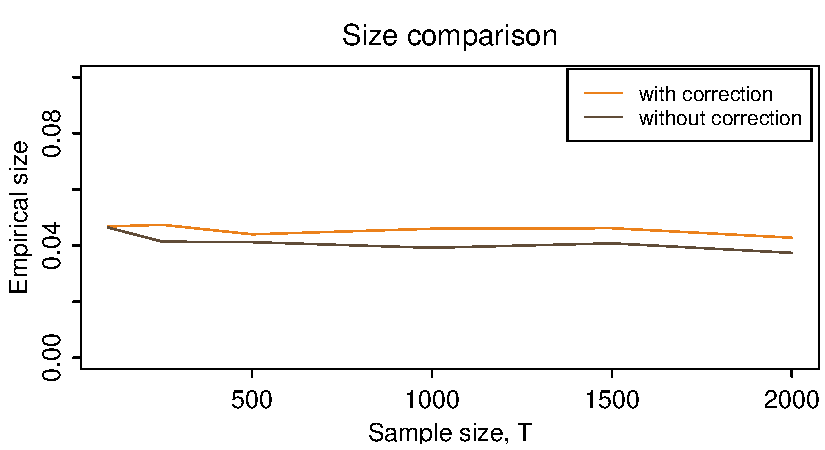
\includegraphics[width=0.95\textwidth]{plots/size_with_correction}
\end{figure}


\hyperlink{frame_critval<4>}{\beamerbutton{Go back}}
\end{frame}



\begin{frame}{Idea behind the additive correction}
Consider the uncorrected Gaussian statistic
\begin{align*}
\Phi^{\text{uncor}} = \max_{(i,j,k)} |\phi_{ijk}|
\end{align*}\pause
and let the family of intervals be \[\mathcal{F} = \big\{[(m-1) h_l, m h_l] \text{ for } 1\le m \le 1/h_l, 1 \le l \le L\big\}\]\pause
Then we can rewrite the uncorrected test statistic as
\begin{align*}
\Phi^{\text{uncor}} = \max_{i, j} \max_{\substack{1 \le l \le L, \\ 1\le m \le 1/h_l}} \Big|\frac{1}{\sqrt{2 T h_l}} \sum\limits_{t=1}^T 1 \Big( \frac{t}{T} \in [(m-1) h_l, m h_l] \Big) (Z_{it} - Z_{jt})\Big|
\end{align*}\pause
$\Rightarrow \quad \max_m \ldots =\sqrt{2\log(1/h_l)} + o_P(1) \to \infty$ as $h \to 0$ and the stochastic behavior of $\Phi^{\text{uncor}}$ is dominated by the elements with small bandwidths $h_l$. \hyperlink{frame_test<4>}{\beamerbutton{Go back}}
\end{frame}

\begin{frame}{Dependence measure}
Following Wu (2005), we define the \textit{physical dependence measure} for the process $\boldsymbol{L}(\mathcal{F}_t)$ as the following:
\begin{align*}
 \delta_q(\boldsymbol{L}, t) = || \boldsymbol{L}(\mathcal{F}_t) - \boldsymbol{L}(\mathcal{F}_t^\prime) ||_q,
\end{align*}
where $\mathcal{F}_t  = (\ldots, \epsilon_{-1}, \epsilon_0, \epsilon_1, \ldots, \epsilon_{t-1}, \epsilon_t)$ and $\mathcal{F}_t^\prime  = (\ldots, \epsilon_{-1}, \epsilon^\prime_0, \epsilon_1, \ldots, \epsilon_{t-1}, \epsilon_t)$ is a coupled process of $\mathcal{F}_t$ with $\epsilon_0^\prime$ being an i.i.d. copy of $\epsilon_0$.\pause

Intuitively, $\delta_q(\boldsymbol{L}, t)$ measures the dependency of $\boldsymbol{L}(\mathcal{F}_t)$ on $\epsilon_0$, i.e., how replacing $\epsilon_0$ by an i.i.d. copy while keeping all other innovations in place affects the output $\boldsymbol{L}(\mathcal{F}_t)$.
\end{frame}

\begin{frame}[label=tech_assumptions]{Technical assumptions}
\begin{enumerate}

\item[$\mathcal{C}1^\prime$] The variables $\varepsilon_{it}$ are independent across $i$ and allow for the representation $\varepsilon_{it} = G_i(\ldots,\eta_{it-1},\eta_{it})$, where $\eta_{it}$ are i.i.d.\ random variables across $t$ and $G_i: \mathbb{R}^\mathbb{Z} \rightarrow \reals$ is a measurable function..

\item[$\mathcal{C}1^{\prime\prime}$]  Define $\Theta_{i, t,q} = \sum\nolimits_{s \ge t} \delta_q(G_i, s)$ for $t \ge 0$. For each $i$ it holds that \linebreak
$\Theta_{i, t,q} = O ( t^{-\tau_q} (\log t)^{-A} )$,  
where $A > \frac{2}{3} (1/q + 1 + \tau_q)$ and \linebreak $\tau_q = \{q^2 - 4 + (q-2) \sqrt{q^2 + 20q + 4}\} / 8q$. \hyperlink{frame_assumptions<3>}{\beamerbutton{Go back}}

\end{enumerate}

\end{frame}

\begin{frame}[label=tech_assumptions_2]{Technical assumptions, part 2}
\begin{enumerate}

\item[$\mathcal{C}3^\prime$] $ \X_{it}$ allow for the representation $ \X_{it} = \boldsymbol{H}_i(\ldots,u_{it-1},u_{it})$ with $u_{it}$ being i.i.d.\ random variables and $\boldsymbol{H}_i := (H_{i1}, H_{i2}, \ldots, H_{id})^\top:\linebreak \mathbb{R}^\mathbb{Z} \rightarrow \reals^d$ being a measurable function such that $\boldsymbol{H}_i(\mathcal{U}_{it})$ is well defined.

\item[$\mathcal{C}3^{\prime\prime}$] Let $\boldsymbol{N}_i$ be the $d\times d$ matrix with $n_{i, kl}= \E[H_{ik}(\mathcal{U}_{i0})H_{il}(\mathcal{U}_{i0})]$ being $kl$-th entry. We assume that the smallest eigenvalue of $\boldsymbol{N}_i$ is strictly bigger than $0$.

\item[$\mathcal{C}3^{\prime\prime\prime}$]  Let $\E [\boldsymbol{H}_{i}(\mathcal{U}_{i0})]=\mathbf{0}$ and $||\boldsymbol{H}_{i}(\mathcal{U}_{it})||_{q^\prime} <\infty$ for some $q^\prime > \max\{ 2\theta, 4\}$, where $\theta$ will be introduced further.
\item[$\mathcal{C}4^\prime$] $\sum_{s=0}^\infty \delta_{q^\prime}(\boldsymbol{H}_i, s)<\infty$ for $q^\prime$ from Assumption $\mathcal{C}3^{\prime\prime\prime}$.
\item[$\mathcal{C}4^{\prime\prime}$] For each $i$ it holds that $\sum_{s=t}^{\infty} \delta_{q^\prime}(\boldsymbol{H}_{i}, s)= O(t^{-\alpha}) $ for $q^\prime$ from Assumption $\mathcal{C}3^{\prime\prime\prime}$ and for some $\alpha > 1/2 - 1/{q^\prime}$. \hyperlink{frame_assumptions<5>}{\beamerbutton{Go back}}

\end{enumerate}
\end{frame}

\begin{frame}[label=tech_assumptions_3]{Technical assumptions, part 3}
\begin{enumerate}

\item[$\mathcal{C}6$] Let $\zeta_{i, t} = (u_{it}, \eta_{it})^\top$. Denote $\mathcal{I}_{it} = (\ldots, \zeta_{i, t-1}, \zeta_{i, t})$, $\mathcal{J}_{it} = (\ldots,\eta_{it-2},\eta_{it-1},\eta_{it})$, $\mathcal{U}_{it} = (\ldots, u_{it-1}, u_{it})$, and $\mathbf{U}_i(\mathcal{I}_{it}) =  \boldsymbol{H}_i(\mathcal{U}_{it})G_i(\mathcal{J}_{it})$. With this notation at hand, we assume that $\sum_{s=0}^\infty \delta_2(\mathbf{U}_i, s)<\infty$.\hyperlink{frame_assumptions<6>}{\beamerbutton{Go back}}
\end{enumerate}
\end{frame}


\end{document}
